

\begin{frame}{DC Optimal Power Flow}
Economic dispatch with quadratic cost function
\begin{alignat*}{3}
\min_{\left(x;\theta,y\right)} && \displaystyle\sum_j \left[  c_2 x_j^2 + c_1 x_j \right.&\left.+ c_0 \right] &   \\
                        && \textstyle \sum_j C^g_{ij} x_j - \sum_e C^b_{ie} y_e          &=d_i       && \forall i \\ 
                 && y_e - b_e \textstyle \sum_i C^b_{ie} \theta_i          &=0         && \forall e \\
                 && y_e &\in \left[ -U_e, U_e \right] && \forall e\\
                 && x_j &\in \left[ G^{min}_j, G^{max}_j \right] && \forall j  
\end{alignat*}
\end{frame}

\begin{frame}{Full JCC Model}
\begin{subequations}
\begin{alignat*}{3}
\min_{\left(x,\beta;\theta,y,\pi,s,z\right)} && \displaystyle\sum_j \left[  c_2 \left(x_j^2 + \beta_j^2 \sD \right)\right. & \left. + c_1 x_j + c_0 \right] &\\
                        && \textstyle \sum_j c^g_{ij} x_j - \sum_j c^b_{ie} y_e          &=d_i       && \forall i \\ 
                 && y_e - b_e \textstyle \sum_i c^b_{ie} \theta_i          &=0         && \forall e\\
                 && y_e &\in \left[ -U_e^\epsilon, U^\epsilon_e \right] && \forall e \\
                 && x_j + \beta_j \sD \eta_g &\in \left[ G^{min}_j, G^{max}_j \right] && \forall j  \\
                 && \textstyle \sum_j \beta_j &=1 &&\\
                 && \pe - \textstyle \sum_j A_{ej} \beta_j   &=0 &&\forall e \\ 
                 && s^2_e - \pi_e^2 \sD + 2 \pi_e \se      &\geq\see &&\forall e \\
                 && z_e - \rho(|y_e|,s_e)  &\geq 0 && \forall e \\
                 && \textstyle \sum_e z_e &\leq \epsilon && 
\end{alignat*}
\end{subequations}
\end{frame}



\begin{frame}{Cost Risk Frontier}
\vspace{-12pt}
\begin{center}
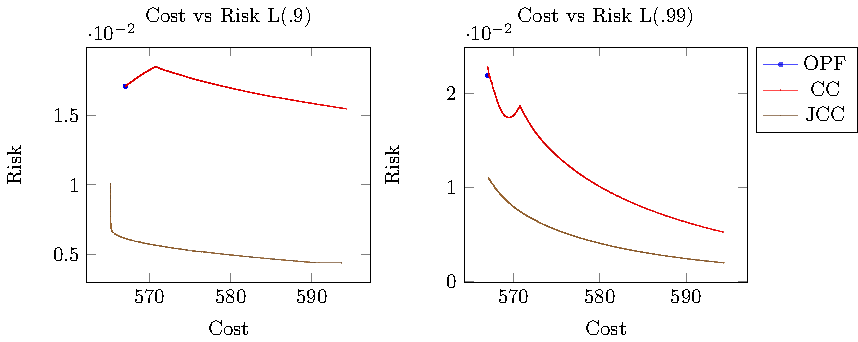
\includegraphics[scale=.8]{fig-costrisk}
\end{center}
\vspace{-12pt}
\bi
\item OPF - single point
\item CC - tighten probabalistic branch constraint from $.5 \rightarrow$ infeasible
\item JCC - tighten system risk from lowest cost $\rightarrow$ infeasible
\ei

\end{frame}


% \begin{frame}{Top 8 Lines}
% \vspace{-15pt}
% \begin{center}
% 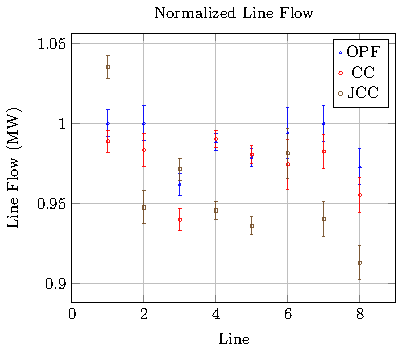
\includegraphics[scale=.9]{fig-top95}
% \end{center}
% \vspace{-5pt}
% \bi
% \item OPF violates 3 constraints 50\% of the time
% \item CC rarely violates constraints
% \item JCC has 1 line above capacity
% \bi
% \item But has less loading on other lines
% \ei
% \ei

% \end{frame}
% \begin{frame}{Congested Line Flows}
% \vspace{-7pt}
% \begin{center}
% 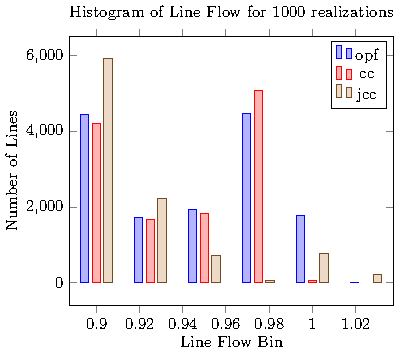
\includegraphics[scale=1.2]{fig-tophisto}
% \end{center}
% \vspace{-10pt}
% \bi
% \item CC and OPF flows pile up at threshold!
% \ei
% \end{frame}

